\documentclass[pdftex,12pt,a4paper]{report}
\usepackage[square,numbers]{natbib}
\bibliographystyle{abbrvnat}
\usepackage[nottoc]{tocbibind}
\setcounter{tocdepth}{4}
\setcounter{secnumdepth}{4}
\usepackage[dvipsnames]{xcolor}
\usepackage[pdftex]{graphicx}
\usepackage{float}
\usepackage{fancyvrb}
\usepackage{dtklogos}
\fvset{xleftmargin=2em}

\usepackage{pgfplots}
\pgfplotsset{width=10cm,compat=1.9}
\usepackage{tikzscale}
\usepackage{pgfplotstable}
\usepackage{booktabs}
\usepackage[font=small,labelfont=bf,tableposition=top]{caption}

\usepackage[utf8]{inputenc}
\usepackage[portuges]{babel}
\usepackage[T1]{fontenc}
\usepackage{times}
%\usepackage{lmodern}
\usepackage[obeyspaces,spaces]{url}
\usepackage[left=20mm,right=20mm,top=25mm,bottom=25mm]{geometry}
\usepackage{titlesec}
\usepackage{mathtools}
\usepackage{amsfonts}
\usepackage{hologo}
%identa 1º paragrafo de capitulos e secções
\usepackage{indentfirst}
\usepackage{url}
%\usepackage{alltt}
\usepackage[]{hyperref}
\usepackage{xspace}

\hypersetup{
%pdftitle={Trabalho 1 - Gestão de Projeto},
%pdfauthor={Bruno Pereira},
%pdfsubject={Investigação Operacional},
%pdfkeywords={keyword1, keyword2}},
bookmarksnumbered=true,     
bookmarksopen=true,         
bookmarksopenlevel=1,       
colorlinks=true,            
pdfstartview=Fit,           
pdfpagemode=UseOutlines, % this is the option you were lookin for
pdfpagelayout=TwoPageRight
		}

\usepackage{minted}
\usemintedstyle{borland}
\setminted{
%frame=lines,
%framesep=2mm,
baselinestretch=1.2,
fontsize=\footnotesize,
linenos, 
breaklines,
breakautoindent=false,
autogobble
}
\usepackage{caption}

\def\BibTeX{{\rm B\kern-.05em{\sc i\kern-.025em b}\kern-.08em
    T\kern-.1667em\lower.7ex\hbox{E}\kern-.125emX}}

\newenvironment{longlisting}{\captionsetup{type=listing}}{}
\def\darius{\textsf{Darius}\xspace}

\def\java{\texttt{Java}\xspace}

\def\pe{\emph{Publicação Eletrónica}\xspace}

\newcommand{\HRule}{\rule{\linewidth}{0.5mm}}


\begin{document}

\begin{titlepage}


\begin{minipage}{0.3\textwidth}
\begin{flushleft} 

\includegraphics[width=1.1\textwidth]{./report/logo.png}
\end{flushleft}
\end{minipage}
\hfill
\begin{minipage}{0.6\textwidth}
\begin{flushright} 

\fontfamily{pag}\selectfont{\large \textsc{Departamento de Informática}\\[0.1cm]
\large \bfseries Mestrado Integrado em Engenharia Informática \\ [0.1cm]
\large \bfseries \textit{Processamento de Linguagens}\\[4mm]
}
\noindent\rule{\textwidth}{0.7mm}
\end{flushright}
\end{minipage}\\[1cm]


\vspace{3cm}


\begin{center}

\fontfamily{pag}\selectfont{\textsc{\Huge Trabalho Prático nº 1}\\[1cm]


{\large \bfseries \emph{Normalizador de ficheiros \hologo{BibTeX}} \\[2cm] }

\vfill
\begin{minipage}{0.4\textwidth}
	\begin{flushleft} 
		\large
	Bruno Pereira\\
\textbf{Aluno nº 72628} 
	\end{flushleft}

\end{minipage}
\begin{minipage}{0.4\textwidth}
	\begin{flushright} 
		\large
	Ricardo Oliveira\\
\textbf{Aluno nº 58657} 
	\end{flushright}
\end{minipage}

\vfill



\vfill

\emph{\large Braga, {\large \today}}
}
\end{center}

\end{titlepage}

\begin{abstract}
	



\end{abstract}

\tableofcontents

\chapter*{Introdução}
\addcontentsline{toc}{chapter}{Introdução} 
\label{intro}


O presente documento visa a documentação do processo de aprendizagem de
especificações em \emph{Flex} e criação de filtros para diversos formatos de
texto. No contexto escolhido, criações de filtros para ficheiros
\hologo{BibTeX}. Numa primeira parte, o objetivo é a criação de uma filtro para
contabilizar as entradas bibliográficas e criar um ficheiro \emph{HTML} com
o resultado. Ficheiros deste género podem crescer muito em tamanho, por vezes
uma contabilização pode ajudar a construir repositórios documentais sobre
determinado assunto. De igual modo, a necessidade de normalização de um
documento deste é importante, porque com o passar do tempo, o acrescentar novas
entradas pode criar desvios de formatação, que pode prejudicar uma pesquisa no
documento pelo nome, por exemplo. Um exemplo de um normalizador deste género
figura na segunda parte (capítulo 2) deste documento.  Além do normalizador, na
terceira parte (cap. 3), é apresentado a elaboração de um filtro para fazer um
\emph{pretty-printing} de um documento \hologo{BibTeX}.  Por último, no quarto
capítulo é apresentada uma ferramenta para criar um grafo com os coautores de
determinado autor, onde os pesos das arestas são a densidade de publicação com
cada coautor.


\section*{Metas e objetivos} 

O ambiente Linux é uma das metas deste trabalho. Existem diversas formas de
fazer determinadas coisas para fazer em Linux, onde cada ferramenta tem o seu
lugar e não faltam ferramentas.  O domínio deste sistema operativo é importante,
dado que, um programador, com conhecimento suficiente sobre este sistema
operativo, tem uma liberdade que falta a outros. De igual modo, dado que as
ações das especificações no \emph{Flex} são programadas em linguagem C, um dos
objetivos passa por refinar e aumentar o conhecimento da linguagem, bem como
aprofundar o conhecimento em estruturas mais complexas. De igual modo,
algoritmos e complexidade são serão revisitados, e a otimização será algo
importante durante a elaboração do trabalho. Pretende-se, portanto, soluções
eficientes. Por último, o grande objetivo é desenvolver a capacidade de escrita
de \emph{ER's} e entender como o funcionamento de processadores de linguagens
regulares funcionam, usando geradores de filtros de texto como o \emph{Flex}.
Deste último objetivo será testemunha este documento.  


\section*{Estrutura do Relatório} 
O relatório está organizado em 4 capítulos: o primeiro capítulo é referente
à alínea \emph{a}, o segundo e terceiros capítulos correspondem à alínea
\emph{b} e o quarto capitulo corresponde à alínea \emph{c}.  Cada capítulo
possui três secções: \emph{Análise do Problema}, \emph{Desenho e implementação
da solução} e \emph{Testes e Resultados}.  Na secção \emph{Análise do Problema}
expõe-se informalmente o problema, contendo conteúdo referentes aos dados,
relações e possíveis abordagens à solução. Na secção \emph{Desenho
e implementação da solução} descrevem-se as especificações e respetivas ações do
\emph{Flex}, \emph{START CONDITION}, estruturas de dados e algoritmos e funções
importantes. Em seguida a secção \emph{Testes e Resultados} apresenta os
resultados e acrescenta uma breve discussão sobre problemas de implementação,
alternativas e sugestões.  Note-se que neste documento, para mostrar
a extensibilidade dos testes, muitos deles estão no \emph{Apêndice}. O documento
encerra com a \emph{Conclusão} onde se avaliará a completude dos objetivos, bem
como observações aos resultados obtidos.






\chapter{Contagens de categorias de um ficheiro \hologo{BibTeX}}
\label{chap:a}

\section{Análise do Problema}
Neste primeiro problema, pretende-se analisar um documento \hologo{BibTeX} e fazer as
contagens das respetivas categorias, tais como artigos, teses de mestrado,
manuais, etc. O resultado tem que constar num ficheiro \texttt{HTML}.


\label{sec:ap:a}

\subsection{Especificação dos requisitos}
\label{sec:spec:a}
Existem pelo menos 14 tipos de entradas bibliográficas no \hologo{BibTeX},
podendo haver algumas extensões ou pacotes que possuam outras --- como por exemplo
o \textsc{Bib}\LaTeX{}.
Note-se que, a distinção entre o formato de ficheiro \hologo{BibTeX}
e o programa \hologo{BibTeX} é importante. O pacote \textsc{Bib}\LaTeX{} pode
ser usado tanto pelo programa \hologo{BibTeX} como não, uma vez que
o \emph{backend} por defeito do \textsc{Bib}\LaTeX{} --- o \emph{biber} ---
suporta o formato de ficheiro \hologo{BibTeX} (\texttt{.bib}). Assim, os
utilizadores do \textsc{Bib}\LaTeX{} podem usar o mesmo ficheiro \texttt{.bib} com
poucas alterações. Em consequência pode-se afirmar, que em cada ficheiro
\texttt{.bib}, todos os tipos de entrada começam com \emph{\@}, ora usam
o \hologo{BibTeX}, ora usem o \textsc{Bib}\LaTeX.


\subsection{Dados}

Os 14 tipos de entradas bibliográficas do \hologo{BibTeX} são:

\begin{itemize}
	\item\textbf{Article      } Um artigo de um jornal ou revista.
    
	\item\textbf{Booklet      } Um livro não publicado por uma editora, mas que
		é impresso e encadernado.
       
	\item\textbf{Book         } Um livro publicado por uma editora.
       
	\item\textbf{Conference   } O mesmo que \emph{Inproceedings}. 
	\item\textbf{Inbook       } Uma parte de um livro, o qual pode ser um capítulo (ou secção ou outro qualquer) e/ou uma série de páginas.
      
	\item\textbf{Incollection } Uma parte de um livro que tem o seu próprio título.
     
	\item\textbf{Inproceedings} Um artigo de uma coleção de \emph{papers} académicos de uma conferência.
   
	\item\textbf{Manual       } Documentação técnica. 
  
	\item\textbf{Mastersthesis} Uma tese de mestrado.
	\item\textbf{Misc         } Qualquer outro documento que não se enquadre em nenhuma
		catgoria.
       
	\item\textbf{Phdthesis    } Uma tese de doutoramento.
      
	\item\textbf{Proceedings  } Coleção de \emph{papers} académicos de uma conferência.
     
	\item\textbf{Techreport   } Um relatório publicado por uma escola ou outra instituição.
    
	\item\textbf{Unpublished  }  Um documento com um autor e título, mas não formalmente
		publicado.

\end{itemize}

Para além destes tipo de entradas existem também as entradas \texttt{@STRING},
\texttt{@PREAMBLE} e \texttt{@COMMENT}, onde a primeira serve para definir
abreviaturas para serem usadas no ficheiro \hologo{BibTeX}, a segundá define
como texto especial deve ser formatado, e a última, serve para incluir
comentários que não devem ser tidos em conta pelo \hologo{BibTeX}.



\section{Desenho e implementação da solução}
\label{sec:des:a}

\subsection{Expressões Regulares}
Antes de se iniciar a descrição, note-se que as \emph{ERs} estão ordenadas de
forma a não haver ambiguidade.


Uma entrada de um ficheiro \hologo{BibTeX} começa sempre com \texttt{@}. De
igual modo, os nomes de tipos de entrada podem ser escritos com maiúsculas ou
minúsculas, bem como podem começar por uma maiúscula, seguidas de minúsculas. Em
suma, não é \emph{case sensitive}. Assim, na especificação do \emph{Flex},
podemos definir uma entrada como um conjunto de caracteres, que começa com
\texttt{@} seguido de uma ou mais ocorrências de caracteres, maiúsculos ou
minúsculos.

Todavia, é necessário especializar a especificação, relativamente às entradas
\texttt{@STRING}, \texttt{@PREAMBLE} e \texttt{@COMMENT}. Também, para os tipos
de entrada bibliográficos é necessário especializar a expressão regular para os
tipos comuns de entradas descritos na secção anterior. A razão desta última
especialização justifica-se apenas por motivos de otimização e eficiência do
filtro, que serão respondidos nas secções seguintes. 

Desta forma temos 4 \emph{ER's}:

\begin{itemize}
	\item Uma expressão regular para capturar ou \texttt{@STRING},
		\texttt{@PREAMBLE} e \texttt{@COMMENT}, da seguinte forma:
\begin{minted}{text}
		\@[Ss][Tt][Rr][Ii][Nn][Gg]
		\@[Pp][Rr][Ee][Aa][Mm][Bb][Ll][Ee]
		\@[Cc][Oo][Mm][Mm][Ee][Nn][Tt]
\end{minted}

A ação nestas expressões regulares é para ignorar.


	\item Uma expressão regular para capturar uma entrada específica, por exemplo:
		\mint{text}|\@[Aa][Rr][Tt][Ii][Cc][Ll][Ee]| para capturar uma ocorrência de
		\texttt{ARTICLE}.

		A ação é contabilizar a ocorrência. Para a contabilização de \emph{ER's}
		deste género, usou-se uma vetor de inteiros, de tamanho 14, em que cada
		posição corresponde a um tipo de entrada.
\newpage

	\item Uma expressão regular para capturar uma entrada genérica, por exemplo:
		\mint{text}|\@[A-Za-z]+| onde o valor capturado é copiado a partir do
		caractere \texttt{@} e inserido numa tabela de
		\emph{hash}, contabilizando repetições.Especificações da tabela de
			\emph{hash} encontram-se na secção seguinte.
	\item Uma expressão regular para ignorar tudo o resto.

\end{itemize}


Por fim, existe a nuance de se fazer a travessia da
tabela de \emph{hash} se houver elementos na tabela.


\subsection{Estruturas de dados}
\label{sec:subsec:es:a}
Escolheu-se uma tabela de \emph{hash} dinâmica que usa o método de
\emph{chaining},
a \texttt{uthash}\footnote{\url{https://troydhanson.github.io/uthash/}} para
utilização neste problema.  Esta possui uma complexidade em termos de tempo
constante na adição, remoção e procura, bem como tem uma melhor gestão de
memória. No entanto, embora haja tabelas mais rápidas, utilizou-se esta tabela
por uma questão de conveniência, dada a simplicidade e ter \emph{performance}
aceitável para este problema.\footnote{\emph{Benchmarking} relativamente
a outras estruturas pode ser encontrado em
\url{http://lh3lh3.users.sourceforge.net/udb.shtml.}}


\section{Testes e Resultados}
\label{sec:ts:a}


\subsection{Resultados}
Para testar o filtro, utilizou-se o ficheiro \hologo{BibTeX} dado como exemplo
em \url{http://www4.di.uminho.pt/~prh/lp.bib}.

O resultado em \emph{HTML} consta no Apêndice~\ref{appendix:a}, na
pág.~\pageref{appendix:a}.

O resultado após ser executado por um \emph{browser} é o que se segue:

\begin{figure}[h!]
	\centering
	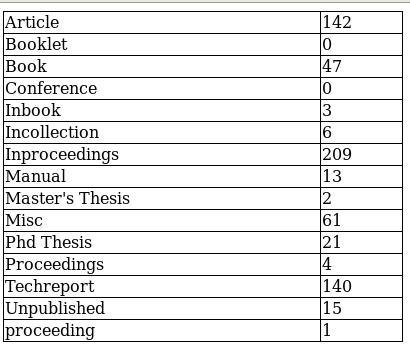
\includegraphics[scale=0.5]{./testes/res_html}
	\caption{Resultado visto no \emph{Firefox}}
	\label{fig:res1}
\end{figure}

A partir do documento que adveio da URL na secção \emph{Resultados}, podemos
constar que não existem entradas que difiram do \hologo{BibTeX}, a não ser
a entrada \emph{proceeding}, e que não existem \emph{Booklets}, nem
\emph{Conferences}. 


\subsection{Alternativas, Decisões e Problemas de Implementação}

Numa primeira implementação, existia uma \emph{trie} para guardar os tipos de
entrada que não pertencessem ao \hologo{BibTeX}. A travessia desta estrutura
é recursiva, embora linear no número de nodos, cada nodo podia ter um
\emph{array} de apontadores de tamanho 256, podendo esse \emph{array} ter poucas
posições ocupadas. De igual modo, a \emph{trie} que estava implementada não
estava otimizada e poderia ter \emph{bugs}. Daí a escolha passar a ser uma
tabela de \emph{hash}. Esta última estrutura, à semelhança da \emph{trie}---
ignorando o tamanho da \emph{string} que compõe a chave ---, continua a ter
tempo constante de inserção, e o \emph{overhead} é menor.

À data de redação deste relatório, chegou-se a conclusão que poder-se-ia ter
escolhido uma tabela de \emph{hash} em \emph{open adressing} ou outra estrutura
otimizada, podendo assim ter um filtro mais eficiente. Futuramente, poder-se-á
tentar utilizar uma estrutura diferente e efetuar mais testes.





\chapter*{Conclusão}
\addcontentsline{toc}{chapter}{Conclusão}
\refstepcounter{chapter}
\label{concl}
Neste documento apresentaram-se as propostas de solução para quatro filtros: um
contador de entradas bibliográficas, um filtro para normalizar um documento,
formatando os nomes dos autores em \emph{N. Apelido} e remoção de chavetas, como
também uma ferramenta de \emph{pretty-printing} e o gerador de grafos em
\emph{Dot} para coautores de um determinado autor e respetiva densidade de
publicação. 

Em relação à aprendizagem do Linux, usaram-se diversas ferramentas para
obtenção de dados e editores de texto, tal como \texttt{grep}, \texttt{sort},
\emph{vim}, \texttt{cat}, \texttt{tac}, \texttt{sed}, entre outros. Um ponto
comum em todos eles foram as \emph{ER} que ampliaram a visão sobre como
trabalhar em Linux.

De igual modo, a utilização das especificações do \emph{Flex} permitiu perceber
melhor as \emph{ERs} e a revisita da linguagem C ajudou a limar algumas arestas.  

A utilização das estruturas poderia ter sido melhor. A escolha da \emph{uthash}
para utilização neste projeto é adequada à sua dimensão, no entanto, existem
estruturas mais eficientes para determinados filtros criados.

De um modo geral, os resultados foram animadores, uma vez que se conseguiu
cumprir com os requisitos do trabalho, de uma forma eficiente. Muito
provavelmente existem melhorias a ser feitas ou algo está parcialmente correta,
ou não o está de todo, no entanto, não se tem conhecimento, dados os testes
efetuados de situações em que os filtros falharam.

Futuramente, poder-se-á estender o projeto a caracteres especiais e tratamento
de caracteres com escape. Uma análise rigorosa poderá por em evidência
alternativas de solução mais eficientes ou mais simples. Testes com outras
estruturas poderão ser efetuados bem como \emph{benchmarking} de cada estrutura
nova aplicada.




\nocite{*}

%\bibliographystyle{alpha}
%
\bibliography{./report/bibs/pl}

\appendix

\chapter{Código do \emph{HTML} da Parte 1}
\label{appendix:a}

\begin{longlisting}
	\inputminted{html}{testes/res_html.html}
	\caption{Ficheiro fonte do exercício 2.1}
	\label{listing:1}
\end{longlisting}




\begin{minted}{c}

#include <stdio.h>
#define N 10
/* Block
 * comment */

 int main()
 {
     int i;
	 
	   // Line comment.
		 puts("Hello world!");
			     
		 for (i = 0; i < N; i++)
		 {
		 puts("LaTeX is also great for programmers!");
		 }
							 
	   return 0;
				
}
\end{minted}


E ainda possível importar diretamente o ficheiro:










\end {document}


